\chapter{Ground Data and Geomagnetic Indices}

	\section{\texttt{groundmag}: Tools for processing and reading ground magnetometer data}
	
	\section{\texttt{SuperDARN}: Simple SuperDARN fitacf reading code}

		\href{https://github.com/mattkjames7/SuperDARN}{https://github.com/mattkjames7/SuperDARN}

		The \texttt{SuperDARN} module is for reading and plotting SuperDARN fitacf files. It is a fairly simple tool, but use with caution because there may be some errors...

		\subsection{Installation}

			This package is not in the PyPI, so manual installation is necessary:
			\begin{minted}{bash}
#clone the repo
git clone https://github.com/mattkjames7/SuperDARN
cd SuperDARN

#build a Python package
python3 setup.py bdist_wheel

#install it (replace 0.1.0 with whatever version is built)
pip3 install dist/SuperDARN-0.1.0-py3-none-any.whl --user
			\end{minted}
			
			Once installed, the directory used to create the Python wheel file can be deleted. It can be uninstalled using \texttt{pip3 uninstall SuperDARN}.

			Before running for the first time, a couple of environment variables need to be set up to tell the module where to look for fitacf files and to say where it is able to store some files:
			\begin{minted}{bash}
#path to where FITACF files are stored 
#(this one is specific to SPECTRE)
export FITACF_PATH=/data/sol-ionosphere/fitacf
	
#path to where this module can create some files
#(this should be a path where you have write access)
export SUPERDARN_PATH=/some/other/path/SuperDARN
			\end{minted}

			This module will not currently run on Windows (as far as I am aware) because it requires the compilation of some C++ code which is not yet cross-platform.

		\subsubsection{Usage}
		
			In ipython, the first time this module is imported, it should attempt to download some files from the \href{https://github.com/SuperDARN/rst}{Radar Software Toolkit (RST)} which help in calculating the coordinates of the fields of view of each radar. These files are created in the path defined be the \texttt{\$SUPERDARN\_PATH} variable.

			\subsubsection{Reading Data}
				There are a few functions within \texttt{SuperDARN.Data} which provide objects containing data:

				\begin{minted}{python}
import SuperDARN as sd
			
#get the data from a single cell (Radar,Date,ut,Beam,Gate)
cdata = sd.Data.GetCellData('han',20020321,[22.0,24.0],9,25)
			
#or a whole beam of data (Radar,Date,ut,Beam)
bdata = sd.Data.GetBeamData('han',[20020321,20020322],[22.0,24.0],7)
			
#data for the whole field of view (Radar,Date,ut)
#in this case, the output is a dict where each key is a beam number
#pointing to a recarray for each beam as produced by GetBeamData
rdata = sd.Data.GetRadarData('han',[20020321,20020322],[22.0,23.0])
				\end{minted}
			
				In the above examples \texttt{bdata} and \texttt{cdata} are \texttt{numpy.recarray} objects, \texttt{rdata} is a \texttt{dict} object containing a \texttt{numpy.recarray} for each beam.
			
				The fitacf data are stored in memory once loaded so that they don't need to be re-read every time the data are requested. To check how much memory is in use and to clear it:
			
				\begin{minted}{python}
#check memory usage in MB
sd.Data.MemUsage()
		
#clear memory
sd.Data.ClearData()
				\end{minted}
			
			\subsubsection{Plotting Data}
			
				There are a bunch of very simple plotting functions, e.g.:
			
				\begin{minted}{python}
import matplotlib.pyplot as plt
			
#create a figure
plt.figure(figsize=(8,11))
			
#plot the power along a beam
ax0 = sd.Plot.RTIBeam('han',[20020321,20020322],[23.0,1.0],9,[20,35],
					Param='P_l',ShowScatter=True,fig=plt,
					maps=[2,3,0,0],scale=[1.0,100.0],zlog=True,
					cmap='gnuplot')
			
#the velocity
ax1 = sd.Plot.RTIBeam('han',[20020321,20020322],[23.0,1.0],9,[20,35],Param='V',
					fig=plt,maps=[2,3,1,0])
			
#velocity along a range of latitudes at a ~constant longitude of 105
ax2 = sd.Plot.RTILat('han',[20020321,20020322],[23.0,1.0],105.0,Param='V',
					fig=plt,maps=[2,3,0,1])
		
#velocity along a range of longitudes at a ~constant latitude of ~70
ax3 = sd.Plot.RTILon('han',[20020321,20020322],[23.0,1.0],70.0,Param='V',
					fig=plt,maps=[2,3,1,1])
			
#some specific cells
beams = [1,5,7,2,8,4,9]
gates = [20,26,33,22,25,21,29]
ax4 = sd.Plot.RTI('han',[20020321,20020322],[23.0,1.0],beams,gates,
					Param='V',fig=plt,maps=[2,3,0,2])
			
#totally different FOV plot
ax5 = sd.Plot.FOVData('han',20020321,23.5,Param='V',fig=plt,maps=[2,3,1,2])
			
			
plt.tight_layout()
				\end{minted}
			
				which should produce figure \ref{FigSDExample}.
			
				\begin{figure}
					\centering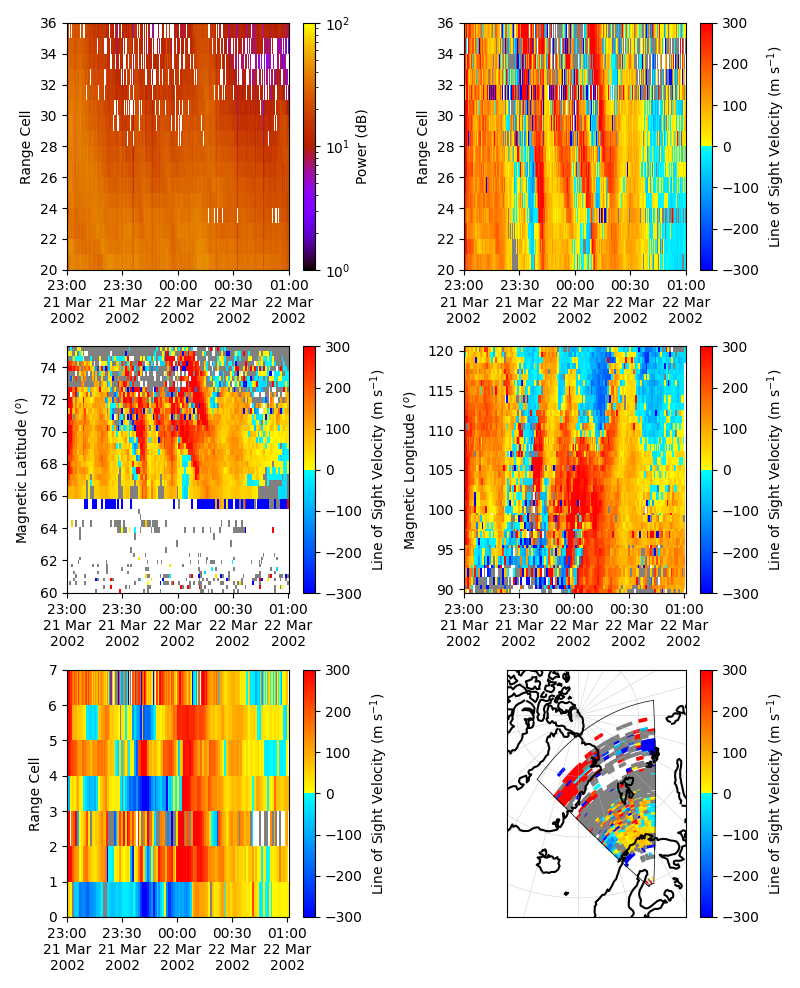
\includegraphics[width=0.8\textwidth]{figures/ch05_sdexample.png}
					\caption{Top left: range time intensity (RTI) plot of backscatter power. Top right: RTI plot of line of sight velocity. Mid left: velocity along a line of cells in magnetic longitude. Mid right: velocity along a range of longitudes. Bottom left: velocity of specific range cells. Bottom right: velocity within the field of view plot. \label{FigSDExample} }
				\end{figure}

			\subsubsection{Fields of View}
			
				These may be wrong. Use with great caution.
			
				The fields of view of each radar are stored as instances of the \texttt{SuperDARN.FOV.FOVObj} objects in memory and can be accessed using \texttt{GetFOV}, e.g.:
			
				\begin{minted}{python}
#get the object from memory
Date = 20020321
fov = sd.FOV.GetFOV('pyk',Date)
			
#use it to retrieve the FOV in mag coordinates
mlon,mlat = fov.GetFOV(Mag=True,Date=Date)
			
#plot it
ax = fov.PlotPolar(Background=[0.0,0.2,1.0],Continents=[0.0,1.0,0.2],
				color='magenta',ShowBeams=False,ShowCells=False,
				linewidth=2.0,Mag=True,Lon=True)
			
#add some cells
beams = [1,5,7,2,8,4,9]
gates = [20,26,33,22,25,21,29]
fov.PlotPolarCells(beams,gates,color='red',fig=ax,Mag=True,linewidth=2.0,Lon=True)
				\end{minted}
			
				The above code should look like figure \ref{FigSDFOV}:
			
				\begin{figure}
					\centering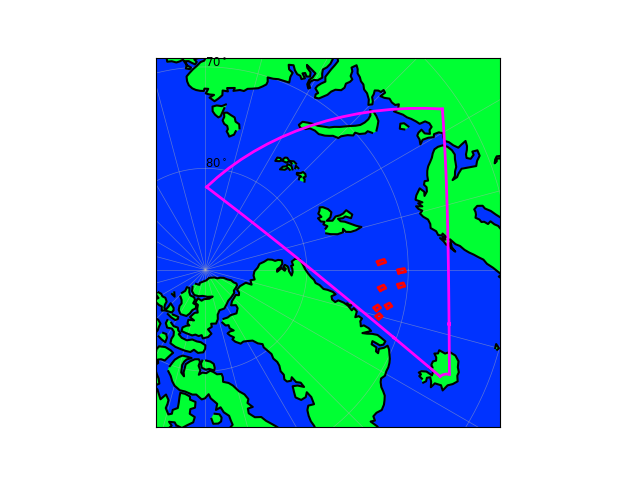
\includegraphics[width=0.5\textwidth]{figures/ch05_sdfov.png}
					\caption{SuperDARN field of view plot with specific cells highlighted.\label{FigSDFOV}}
					
				\end{figure}
			


	\section{\texttt{kpindex}: Download the latext Kp indices}

	\section{\texttt{pyomnidata}: Download the latext OMNI and solar flux data}

	\section{\texttt{smindex}: Read the SuperMAG indices}




